% !TeX root = ../main.tex
% Add the above to each chapter to make compiling the PDF easier in some editors.

\chapter{Background}\label{chapter:background}

This chapter discusses the relevant background knowledge required to understand the remainder of this work.

\section{Trusted execution environment}

% Motiviation for TEE's

One of the core security concepts of operating systems are the privilege levels of processes~\cite{Linden1976}. Thereby, processes are protected against other processes with the same or lower privilege level. However, they are not protected against more privileged processes~\cite{Bratus2009}. This bears problems for example for cloud computing and edge computing. In cloud computing, other services, the hypervisor, or the cloud provider in general could potentially access sensitive data of the cloud tenant~\cite{Nimgaonkar2012}. In edge computing, the edge applications deal with plain text data, while they are potentially running on insecure edge devices~\cite{Ning2018}. Hence, protection against more privileged processes is desired.


% What TEE's are

The \acf{TEE} is a technology defined by GlobalPlatform\footnote{\url{https://globalplatform.org/}} as an integrated hardware extension to processors. By that, the execution environment is separated into the \ac{REE} and the \ac{TEE} by hardware.
The \ac{REE} runs commodity software, e.g., a Linux-based operating system with user applications.
The TEE is an isolated tamper-resistant execution environment that guarantees the authenticity of the executed code, and the integrity of runtime states, e.g., memory~\cite{Sabt2015}.
Since a \ac{TEE} is integrated into the processor, there is no separate chip required.
% The TEE allows code to be executed and memory separately to be used on a device in a hardware-protected manner that ensures a high level of confidentiality and integrity.
Moreover, the \ac{TEE} commonly follows the same user and kernel space separation as a rich OS\@. The kernel space is running a trusted OS, and the user space is running the trusted applications. 
It focuses on resisting software-based attacks generated in the \ac{REE}, however, also protects against some hardware attacks~\cite{GPSysArch}.


% Differences to previous technologies

Previous, mostly software-based technologies ensure confidentiality and integrity protection of data-in-transit and data-at-rest~\cite{Pecholt2022}, while a \ac{TEE} additionally protects data-in-use in hardware~\cite{Pecholt2022, Lee:EECS-2022-96}.
% For example, smart cards are commonly used to store keys to identify users and to encrypt data-at-rest~\cite{Arthur2015}.

% Figure explanation

\autoref{fig:tee_motivation} illustrates the motivation. In the traditional architecture, i.e., without a TEE, if an attacker compromises the \ac{REE} the full system is affected. With a \ac{TEE}, the attacker is limited to the \ac{REE}, while the \ac{TEE} continues to protect the secure assets, such as encryption keys. This results from the observation that the attack surface of a rich OS is much larger than that of a trusted OS, e.g., due to its network connectivity and the high dynamics of software installations, while the attack surface of a trusted OS is rather small and has tightly controlled interfaces.

\begin{figure}[htpb]
  \centering
  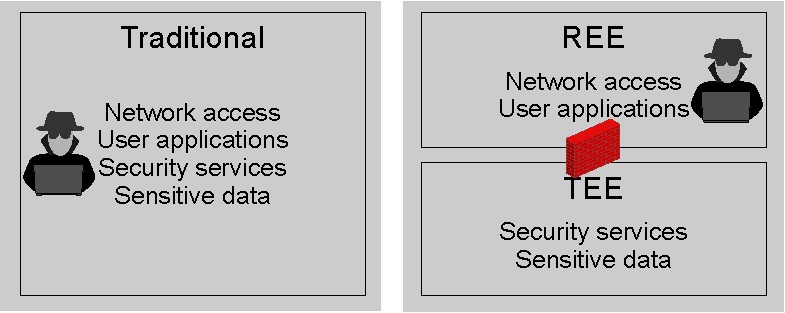
\includegraphics[width=0.8\linewidth]{figures/TEE-motivation.pdf}
  \caption{Comparison between a traditional architecture and an architecture separating the REE and TEE\@. This illustrates the motivation of a TEE\@.}\label{fig:tee_motivation}
\end{figure}


\subsection{Arm TrustZone}

One such \ac{TEE} is Arm's TrustZone~\cite{ARM09, Ngabonziza2016}. It partitions all software and hardware resources of the containing system into the \ac{NW} and the \ac{SW}, as shown in \autoref{fig:arm_trustzone_arch}. The secure monitor is triggered by the dedicated instruction Secure Monitor Call (SMC), which then manages the context switches between the \ac{NW} and the \ac{SW}.
While the \ac{SW} can access the resources of the \ac{SW} and the \ac{NW}, the \ac{NW} is restricted to its own assigned resources.
Since Arm is the dominant processor architectures for IoT devices with a market share of 86\,\%~\cite{eclipse}, many of the approaches in this field of research use Arm TrustZone~\cite{Valadares2021}.

\begin{figure}[htpb]
  \centering
  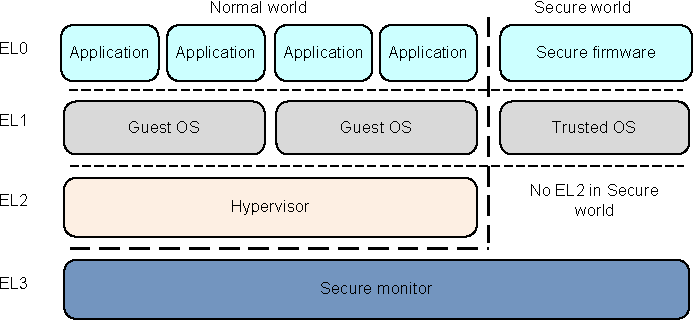
\includegraphics[width=0.8\linewidth]{figures/arm-trustzone-arch.pdf}
  \caption{The architecture of Arm TrustZone for AArch64 \cite{TZArch}. The exception levels (EL) indicate the privilege levels.} \label{fig:arm_trustzone_arch}
\end{figure}


Our implementation also leverages TrustZone to enable the execution and the remote attestation of an fTPM\@.

\subsection{Further TEE technologies}

Other \ac{TEE} technologies are Intel Software Guard Extensions~(SGX), and AMD Secure Encrypted Virtualization~(SEV), in the future also Intel Trusted Domain Extensions~(TDX), and Arm Confidential Computing Architecture~(CCA). Since we focus on the implementation of our concept with Arm TrustZone, we do not go into detail about these other technologies here. However, since our concept is not tied to Arm processors and can also be applied to others, they are mentioned for the sake of completeness.

% TrustZone, Trusted applications are not isolated -> they need to trust each other

% From TrustZone section in TPM book: Peripherals can be switched between the NW and SW by configuring the system monitor to forward the peripheral interrupts only to the assigned world, because some peripherals might need to be secure only temporarily.

% static: Arm TZ
% dynamic: Intel SGX, TDX, AMD SEV


\section{Attestation}

% According to the Cambridge Dictionary an attestation is ``a formal statement that you make and officially say is true''.

According to NIST SP 1800--19B~\cite{Bartock2022} an attestation is ``the process of providing a digital signature for a set of measurements securely stored in hardware, and then having the requester validate the signature and the set of measurements.''
Specifically in our context, attestation is a mechanism for software to prove its identity.
In the following, the two types are discussed.


\subsection{Local attestation}

Local attestation is a procedure in which the state of a computer is measured, whereby the measurement result does not leave the computer but is used directly by a local component. One such example is a \ac{TPM} that releases data, e.g., an encryption key, only when the computer is in a known state. This feature is known as sealing~\cite{tpm}.

% Local attestation enables assertions between two environments on the same system~\cite{Anati2013InnovativeTF}. The claim of an environment can be verified by another environment, usually with the help of message authentication codes (MAC)~\cite{Menetrey2022}. For example, Intel SGX uses this mechanism to establish assertions between two enclaves~\cite{Anati2013InnovativeTF}.

% Example is the sealing functionality of the TPM. It only releases information if the state of the system is as expected.

\subsection{Remote attestation}

% Doctor analogy
% A company conducts a remote attestation if a worker provides a sickness attest to a company.
% In this scenario, the worker is the attester/prover, the doctor is the verifier, and the company is the relying party.
% Trust in the doctor is established via his medical license, rooted most commonly in a government agency who only certifies doctors which are declared trustworthy since they fulfilled a list of requirements, like succeeding a medical education. 

\begin{figure}[htpb]
  \centering
  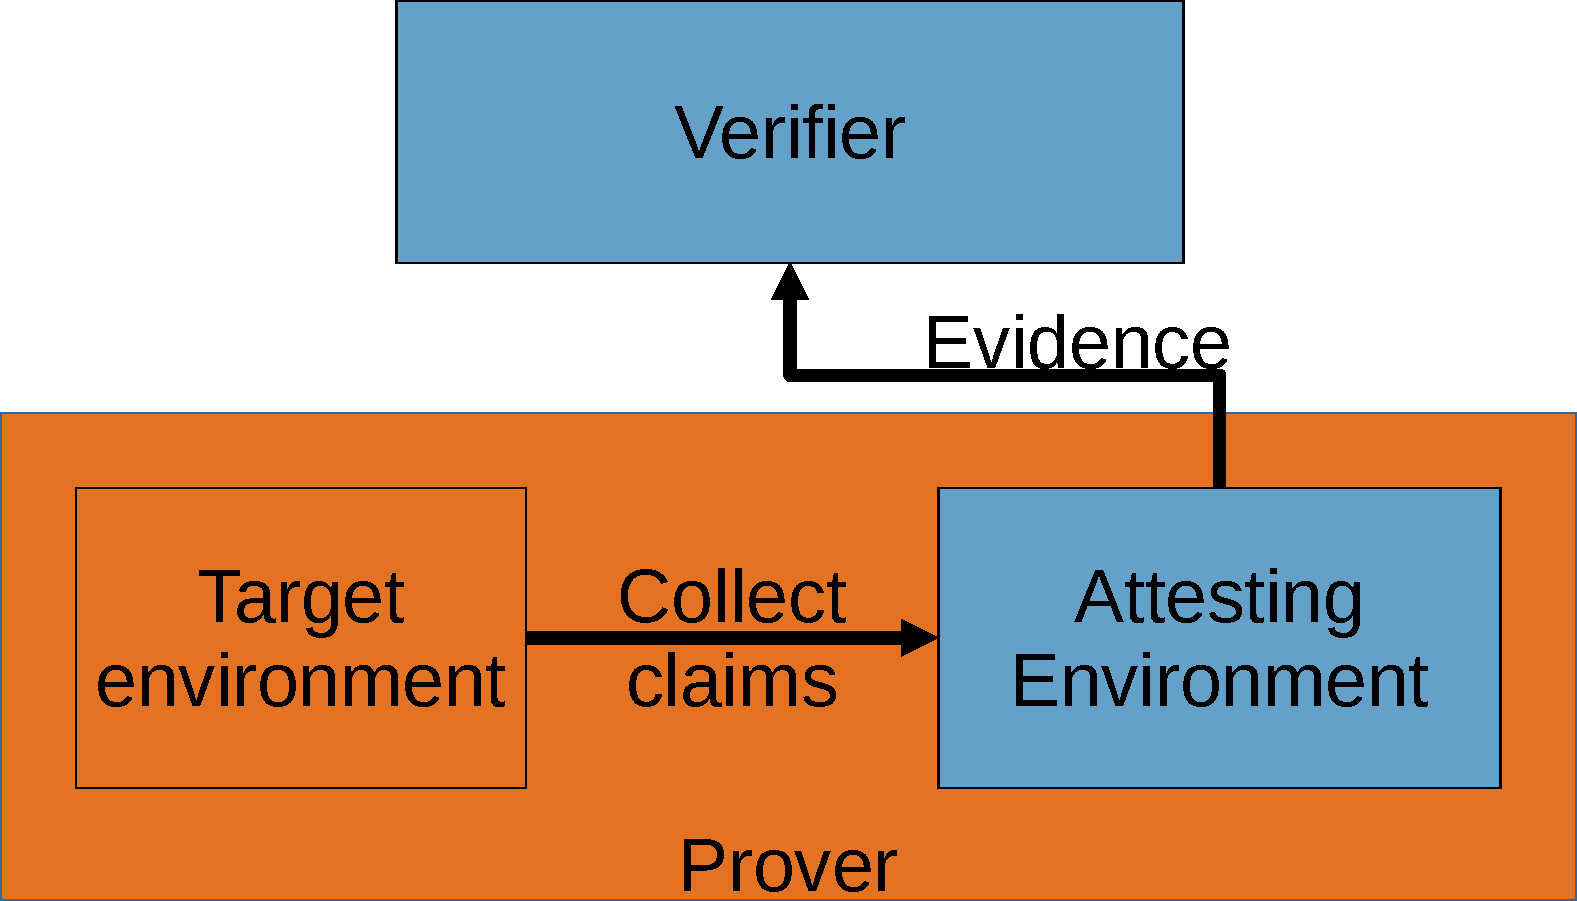
\includegraphics[trim={0 5cm 0 0}, width=0.5\linewidth]{figures/remote_attestation.pdf}
  \caption{Data flow of remote attestation \cite{rfc9334}. Initially, only the blue areas are trusted by the verifier. After the attestation, the verifier also trusts the target environment.} \label{fig:ra}
\end{figure}


In contrast to that, the measurement, usually called evidence, leaves the measuring machine, and is transmitted to a remote verifier for a remote attestation. This involves cryptographic primitives to establish trust into this evidence which is generally transmitted through an untrusted network.

Remote attestation is a challenge-response protocol initiated by a remote attestor.
\autoref{fig:ra} depicts a simplified overview of the data flow of a remote attestation.
The process is initiated by a remote trusted party (called ``verifier'') to verify that a target environment on the end-device (called ``prover'') has not been tampered with~\cite{Menetrey2022, Coker2011}. This challenge contains a nonce, enforcing a fresh response.
The response must be an evidence of the challenged system that it is trustworthy. To build that, an attesting environment on the prover device generally inspects the following properties of a program: (i) its code and data has been correctly loaded into memory for execution, and (ii) its data has not been maliciously modified at runtime.

The attesting environment acts a root of trust for measurements (SRTM).
It is required on the prover because at least one trusted component is necessary to conduct trusted measurement of the prover. In many cases, the SRTM is running within the TEE, since thereby it is better protected from attacks.

It typically consists of two parts~\cite{McCune2008}.
(i) The attestation, and (ii) the accompanying establishment of a secure channel.
In this work, we focus on the first step.

A remote attestation procedure can also be divided into two categories, implicit and explicit attestation.
In implicit attestation, the state of the verifier is implicitly inferred from the fact that the verifier has control over a signing key that is only accessible in a known state.
With explicit attestation, the state of the device is explicitly described in the evidence.

\section{Trusted Platform Module}\label{sec:tpm}

The \ac{TCG}\footnote{\url{https://trustedcomputinggroup.org/}} published the first TPM specification (v1.2) in 2009~\cite{ISO11889}, and the most current specification (v2.0 Revision 01.59) ten years later in 2019~\cite{tpm}.
% First v2.0 version was much earlier
It describes a cryptographic coprocessor that increases trust in the host platform. Specifically, this means that the platform exhibits the expected behavior and that this behavior can be trusted.
For that, the TPM maintains a separated state from the host platform, which enables the TPM to take measurements of the host platform.
It is also a passive device, meaning it only does something when prompted.
\autoref{tab:tpm_use_cases} summarizes the main features of TPMs.

\begin{table}[htpb]
  \caption[TPM features]{TPM main features and according short explanations.}\label{tab:tpm_use_cases}
  \centering
  \begin{tblr}{Q[l,m] Q[l,m]}
      \toprule
      Feature & Explanation \\
      \midrule
      Device identification    & {Identify a machine, e.g., before\\ granting it access to resources} \\
      % Encryption               & Encrypt files on a device \\
      True Random Number Generator  & Seed key generation algorithms \\
      Key Storage              & Store secret keys \\
      Platform Configuration Registers & {Store measurements of system components} \\
      Sealing                  & {Bind access to data to state of host system\\i.e., specific PCR values} \\
      \bottomrule
  \end{tblr}
\end{table}


Each key created and stored on a TPM is part of one of four hierarchies.
The following list shows the official names of the hierarchies as defined in the TPM specification~\cite{tpm}, some alternative names behind them in brackets, as they are sometimes referred to, and the intended use-case of the hierarchies~\cite{Arthur2015}.
\begin{itemize}

  \item{Storage hierarchy (owner hierarchy);\\
  This is the hierarchy mainly used by the end user of a TPM, e.g., to store SSH keys.}

  \item{Endorsement hierarchy;\\
  Therein are stored privacy-sensitive keys, most importantly the EK.}

  \item{Platform hierarchy;\\
  It is intended to be used by early boot code like the UEFI\@.
  For example, the UEFI can store its configurations under this hierarchy.}

  \item{Null hierarchy (ephemeral hierarchy);\\
  Used for temporary keys, e.g., when the TPM is being used as a cryptographic coprocessor.
  Keys in this hierarchy are discarded when the TPM is restarted.}

\end{itemize}

\begin{figure}[htpb]
  \centering
  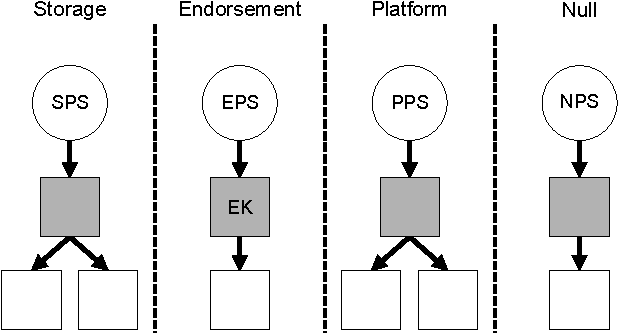
\includegraphics[width=0.8\linewidth]{figures/tpm-hierarchies.pdf}
  \caption{The source of entropy of the keys generated in a TPM for each hierarchy. Circle: primary seed, e.g., the storage primary seed~(SPS); gray rectangle: primary key, e.g., the endorsement key~(EK); white rectangle: ordinary key.
  }\label{fig:tpm-hierarchies}
\end{figure}


The hierarchies are separated in order to provide actors with finely granular access to the TPM\@.
For example, a privacy administrator can only have access to the endorsement hierarchy, while the end user only has access to the owner hierarchy.
They possess different behaviors as well.
The Null hierarchy, for example, cannot be restricted, while the Platform hierarchy is unlocked each time the TPM is restarted, i.e., has an empty password, and is intended to be locked by the early boot code by setting a password only known to the early boot code.

A TPM derives keys from two parameters, a source of object entropy and a key template.
The object entropy for a primary key comes from the according primary seed, for an ordinary key from the parent key, as depicted in \autoref{fig:tpm-hierarchies}.
Note that ordinary keys can also have children, so there can be more levels than in \autoref{fig:tpm-hierarchies}.

A template contains metadata of the key, such as the type of key, e.g., RSA, and the object attributes.
The attributes assign for example whether the key can be used for encryption or signing.
Keys can also be restricted, which restricts the key to be used with data generated by the TPM~\cite{tpm}.
For signing keys, this prohibits the TPM to sign data with it which seems to be generated by the TPM, but are actually not.
This prevents an attacker from asking the TPM to sign an artificially constructed quote.
And restricted encryption keys can only be used to encrypt TPM generated data like keys.

% \autoref{eq:ek}.
% \begin{equation}
%     \label{eq:ek}
%     key = KDF(entropy\_source,\ key_{template})
% \end{equation}

The \acp{PCR} are the fundament for the remote system attestation. They are one-way registers, which values can never be written to an exact value, but only be extended.
This operation is known as `hash extend'~\cite{Arthur2015}.
Its design prohibits the removal of extensions, which would cause the TPM to forget a measurement, and the arbitrary writing of values, which would overwrite any previously conducted measurements.
A PCR value holds a hash representing the platform state.
Thereby, a remote verifier can request a so-called `quote' from the TPM on the host in question.
A quote contains the hash of all requested PCR values and is digitally signed.
Typically, a TPM contains 24 PCR registers, as defined as the minimum by~\cite{tcgPcClient}, with the lower PCR values representing the system boot process and the higher ones representing the events after the kernel is booted~\cite{Arthur2015}.
%\autoref{tab:pcr_usages} shows the components each PCR value represents as specified by the TPM PC Client specification~\cite{tcgPcClient}.
The fixed length of the \ac{PCR} values is important for the memory-constrained nature of TPMs~\cite{Arthur2015}.

The PCR value at index \(i\) can only be modified, i.e., extended, by adding together the currently contained hash value and the new hash, as depicted in \autoref{eq:pcr_extend}~\cite{tpm}. For the sake of correctness, it should be noted that not every PCR is initialized with zero, as implied in the equation. For example, the TPM PC Client Platform specification~\cite{tcgPcClient} defines that PCRs 1--15 are initialized with all bits set to 0, while PCRs 17--22 are initialized with all bits set to 1.
\begin{equation}
  \label{eq:pcr_extend}
PCR(i)_{t=0} \coloneqq 0,\quad PCR(i)_{t+1} \coloneqq hash(PCR(i)_t\ \Vert\ new\ value)
\end{equation}

%\begin{table}[htpb]
  \caption[PCR table]{The PCR register usages as defined by the TPM PC Client specification \cite{tcgPcClient}.}\label{tab:sample}
  \centering
  \begin{tblr}{Q[c,m] Q[l,m]}
      \toprule
      PCR Index & Usage \\
      \midrule
      0    & {SRTM, BIOS, host platform extensions,\\ embedded Option
      ROMs and PI Drivers} \\
      1    & Host platform configuration \\
      2    & UEFI driver and application code \\
      3    & UEFI driver and application configuration and data \\
      4    & UEFI Boot Manager code (usually the MBR) and boot attempts \\
      5    & {Boot Manager Code configuration/data and GPT/partition table} \\
      6    & Host platform manufacturer specific \\
      7    & Secure boot policy \\
      8-15 & Defined for use by the static OS \\
      16   & Debug \\
      23   & Application support \\
      \bottomrule
  \end{tblr}
\end{table}


% Sealing (local attestation)
% EKcert, EK = Unique ID, key in TPM, used for validation
% Binding to TPM (EK)
% Core Root of Trust of Measurement: BIOS extension, trusted hashing
% Attestation: TPM confirms measured state

TPM~1.2 is limited to SHA-1 hashes which are considered broken~\cite{cryptoeprint:2005/010, Wang2005, Stevens2017}. Although the SHA-1 uses in TPM~1.2 were analyzed to be not affected~\cite{sha1tpm12}, cryptographic algorithms only become weaker over time~\cite{Arthur2015}. In reaction, TPM~2.0 offers crypto-agility and allows newer algorithms such as SHA-256. In general, TPM~2.0 is more flexible, and is always turned on, while a TPM~1.2 needed to be turned on manually. Also, TPM~2.0 is more consistent across different implementations because of broader specifications.
TPM~2.0 is the focused version nowadays, e.g., Microsoft recommends TPM~2.0 over TPM~1.2 because of security advantages~\cite{micrec}, and also requires TPM~2.0 for Windows~11 with SHA-256 PCR registers~\cite{win11req}.

% SRTM (from the beginning, what we use)
% DRTM (at any point of time, established by HW extensions, root of trust is e.g. Intel microcode/Hardware)

\begin{figure}[htpb]
  \centering
  \begin{subfigure}{0.49\textwidth}
    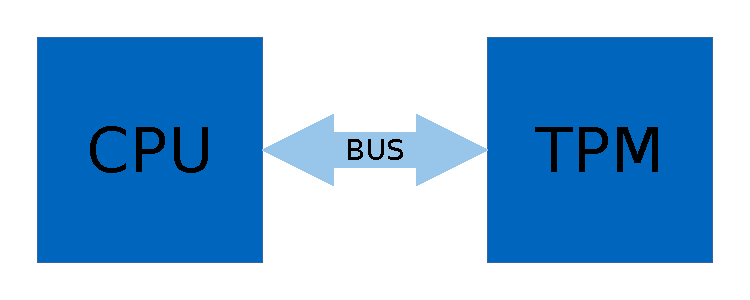
\includegraphics[width=\linewidth]{figures/dTPM.pdf}
    \caption{Discrete TPM} \label{fig:dtpm}
  \end{subfigure}%
  \hspace*{\fill}   % maximize separation between the subfigures
  \begin{subfigure}{0.49\textwidth}
    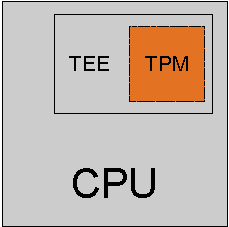
\includegraphics[width=\linewidth]{figures/fTPM.pdf}
    \caption{Firmware TPM} \label{fig:ftpm}
  \end{subfigure}%

  \begin{subfigure}{0.49\textwidth}
    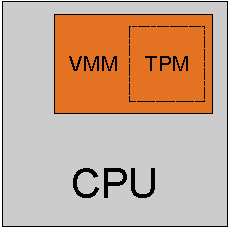
\includegraphics[width=\linewidth]{figures/vTPM.pdf}
    \caption{Virtual TPM} \label{fig:vtpm}
  \end{subfigure}%

  \caption{Schematic illustration of the different TPM types in their pure form. Blue: Hardware, Orange: Software.} \label{fig:tpm_types}
\end{figure}


There are three types of TPMs, as illustrated in \autoref{fig:tpm_types}. They all offer the same functionality, but with different security guarantees and performance characteristics.



\subsection{Discrete TPM}

This is the classical form of a TPM\@. It is a dedicated piece of hardware, connected to the CPU via a bus. It is designed and manufactured to be highly temper-resistant against hardware attacks.
The TPM specifications~\cite{tpm, tcgPcClient} do not demand a specific bus system, however, they define the interfaces between the TPM and the following bus systems: LPC, I\textsuperscript{2}C, and SPI\@.


\subsection{Firmware TPM}

% Generally more secure? According to https://arxiv.org/pdf/2304.14717.pdf, yes
% But TEEs are also tamper-resistant, aren't they? Maybe not as much as dTPMs.

% https://www.microsoft.com/en-us/research/wp-content/uploads/2016/02/msr-tr-2015-84.pdf talks about differences in security

An fTPM~\cite{Raj2015, 197213} is executed directly by the CPU within a \ac{TEE}.
This isolates it from the \ac{REE}, which means that even the operating system in the REE cannot arbitrarily access the memory of the fTPM\@.
The \ac{REE} can only send commands to the fTPM via controlled interfaces.
These commands are piggybacked by calls from the \ac{REE} to the fTPM in the \ac{TEE}.
The trend is moving towards fTPMs, which can also be seen by the increasing efforts to bring an fTPM to the RISC-V processor family~\cite{Boubakri2021}.

As of now, a fTPM is strictly bound to the processor manufacturer, such that you can trust the underlying firmware as well which is provisioned by the manufacturer, e.g., Intel, too. For example, common implementations are the Intel® Platform Trust Technology~(Intel PTT)~\cite{intelProcessorSecurity}, and AMD's Secure Processor~(AMD-SP), with the latter being an Arm-based coprocessor on the die with Arm's TrustZone~\cite{Khalid2020}.
Running on the main processor, e.g., a fully-fledged Arm Cortex core, entails advantages and disadvantages.

% Disadvantages

A disadvantage is that running on the same processor as the rest of the system means less isolation from the remaining system, while a \ac{dTPM} brings its own processor, memory, and storage that is completely isolated from the main system. 
Also, \acp{fTPM} cannot provide true RNG, since hardware is required for that~\cite{Stipcevic2014}.
% Well, they can if the fTPM RNG is connected to a hardware RNG. I think I even remember that in some paper they tried to harden fTPMs just by doing exactly this.
Furthermore, they are started later in the host's boot chain than a dTPM that is accessible from the beginning.
This has the consequence that the measurements of the components booted before the fTPM have to be cached and later be forwarded to the \ac{fTPM} as soon as it is available.
Arm's Trusted Firmware-A\footnote{\url{https://www.trustedfirmware.org/}}, which is the Arm's reference implementation of software in the \ac{TEE}, protects this cached event log by keeping it in secure memory~\cite{tf-a-measured-boot}, i.e., memory which is only accessible in the \ac{TEE}. 
Last, fTPMs depend on more components for its security than single-component dTPMs, e.g., the hardware-provided isolation between the \ac{REE} and the \ac{TEE}, and the boot chain.

% Advantages

However, since they require only a TEE which is mostly already available at currently used processors, they are cheaper for manufacturers as they require less extra hardware.
In addition, TPM processors are weak~\cite{Goh2013, Raj2015}.
Raj et al.~\cite{Raj2015} and Cheng et al.~\cite{Cheng2020} independently concluded that firmware TPMs executed on main processors are generally much faster than \acp{dTPM}.
They are also a viable option for adding TPM functionality to older devices through software updates rather than hardware replacements, which is particularly valuable in times like the recent chip supply shortage~\cite{Voas2021, casper2021}.


% \begin{table}[htpb]
%   \caption[ftpmdownsides]{Advantages and disadvantages of fTPMs.}\label{tab:tpm_comparison}
%   \centering
%   \begin{tblr}{Q[l,h] Q[l,m]}
%     \toprule
%     Advantages      &  Disadvantages \\
%     \midrule
%     Faster          &  No perfect RNG \\
%     Easier update   &  {Launched later in boot chain.\\ Cannot measure hashes of preceding boot components.} \\
%     \bottomrule
%   \end{tblr}
% \end{table}


\subsection{Virtual TPM}

A vTPM is a software-based TPM provided by a hypervisor for one of its managed virtual machines~\cite{268868}.
The vTPMs can be realized fully in software~\cite{268868}, or backed by dTPMs~\cite{Liu2010}.
The hypervisor can provide a (theoretically) unlimited number of vTPMs.
For the virtual machines it seems that they have exclusive access to their own private TPM, even though all vTPMs are managed by the same hypervisor.
A characteristic feature of virtual resources are their migration capabilities, i.e., they can be suspended and later continued on another machine.
Virtual TPMs support this as well.
Note that a vTPM does not inherently have its own security properties, but that these depend entirely on the vTPM implementation of the hypervisor.


\section{Secure Boot and Measured Boot}

When the system is started, the root component, e.g., from ROM, is executed. This subsequently launches the next component, and so forth. This boot structure is called the boot chain. Typically, the first component turns on the memory, the second stage initializes the platform, and finally, the last stage boots the operating system~\cite{Yao2020}.

Secure Boot~\cite{Hendricks2004, UEFI, Frazelle2020} is verifying components of the boot chain directly at boot-time. For that, the boot component is equipped with a public key. With that, they verify the digital signature of the respective subsequent component, before handing over the execution. This ensures the authenticity of the boot components. Alternatively, merely the hashes of the components can be measured and compared with known values, which only ensures integrity and not authenticity. The first boot component, usually stored in ROM, needs to be trusted without verification, i.e., it acts as the root of trust. However, Secure Boot does not prevent downgrade attacks, since only the authenticity, but not the concrete versions of boot components are verified~\cite{272306}. Hence, further defenses like Measured Boot have been designed.

% Secure Boot is a concept of UEFI~\cite{UEFI, Frazelle2020} doing local attestation of components of the boot chain directly at boot-time. Each stage measures the subsequent component before handing over the execution, and compares it with the expected value. This expected value is signed, i.e., a signature, and each boot binary contains its own signature. Providing a signature verifies not only the integrity, but also the authenticity of the component's source. The boot process is canceled as soon as deviations are detected.
% For this purpose, boot chain binaries are first signed and then, deployed universally. Hence, the binaries are not bound to the platform and can be considered portable in this context.

Measured Boot~\cite{tcgMeasuredBoot} is a concept that is implemented in interplay with a TPM\@. It allows remote attestation to a later time. Just as with Secure Boot, each boot component hashes the subsequent component. However, instead of directly locally verifying the measured value, the hash value is passed to the TPM to extend a \ac{PCR} value. As described in \autoref{sec:tpm}, these values can be used by a remote attestor to verify the state of the software on the system. The goal is to detect manipulated system configurations.

Secure Boot and Measured Boot are often used in conjunction.

\section{Device Identifier Composition Engine}

% Primer
\ac{DICE} was originally proposed by Microsoft as part of their Robust Internet-of-Things (RIoT) architecture~\cite{England2016}. In 2017, the DICE specification was published by \ac{TCG}~\cite{tcg-microsoft-tpm}, of which Microsoft is a member.
Its purposes are to detect firmware tampering and enable device identification for a remote party, while its main attribute is its minimal hardware requirements.

% Measurement chain

DICE operates on a boot process layered into components~\cite{dice-layering-arch}.
Later components are typically more feature rich and complex than earlier ones.
Each component is measured prior becoming active by the preceding component.
Great care must be taken to ensure that the identity of the measured and thereafter executed component is consistent~\cite{Hristozov2022, Carpent2018}.
The union of all security-relevant components of a device form its Trusted Computing Base (TCB).
Their identities are called TCB Component Identifier (TCI).
They are usually the hashes of the according firmware binary, but could also consist of a hardware product identifier.

% Hardware requirements

The first component is the DICE itself, which consists of software and hardware. The DICE specification~\cite{dice-hardware-reqs} states the three hardware requirements, the DICE layer 
\begin{enumerate}
  \item has to store a read-only Unique Device Secret (UDS),
  \item has exclusive access to the UDS,
  \item and is immutable.
\end{enumerate}
These requirements can be justified intuitively.
(1) The UDS must be read-only and unique to the device to enable a base for long term identification.
(2) The DICE layer reads and uses the UDS, and then needs to erase the UDS from memory while preventing other components from retrieving this secret during the power-on time.
Otherwise, other entities can forge measurement or identification values. This lock mechanism can, for example, be realized with eFuses~\cite{dice-hardware-reqs}.
(3) Moreover, the misbehavior of the DICE layer cannot be detected since it is not preceded by anything that could measure it, i.e., it is the root of trust.
Therefore, it must be immutable so that it remains in the trusted state in which the manufacturer provided it.

% What is the CDI, and what is it derived from?

While the UDS is exclusive to the DICE layer, each other component retrieves a Compound Device Identifier (CDI) from its previous component.
The CDI of each layer depends on two variables combined in a one-way function (OWF).
(i) The own TCI, binding the CDI to the current layer's identity, i.e., the hash of itself, and (ii) the CDI of the previous layer, making each CDI depending on the identities of all previous component identities.
Therefore, if any component is modified, this reflects in the permutation of the CDIs of all subsequent components, as implied by \autoref{eq:dice_cdi}.

% CDI protection and further uses

Just as the DICE layer must ensure to have exclusive access to the UDS, each later layer must ensure to have exclusive access to its CDI\@.
The layers can derive further secrets using their CDI as a seed, such as the Device ID key pair (\autoref{eq:dice_deviceID}) or an alias key pair (\autoref{eq:dice_alias}).

\noindent
\begin{minipage}{\linewidth}
\begin{align}
  \label{eq:dice_cdi}
  CDI_n &= \underbrace{UDS\ \circ\ TCI_0}_{CDI_0}\ \circ\ \ldots\ \circ\ TCI_n\\
  \label{eq:dice_deviceID}
  DeviceID\_KeyPair &= KDF(CDI_0)\\
  \label{eq:dice_alias}
  Alias\_KeyPair_n  &= KDF(CDI_n)
\end{align}
where \(a \circ b = OWF(a,\,b)\), \(\circ\) being a left-associated operator, and \(KDF\) being a key derivation function.
\end{minipage}
\vskip0.4\baselineskip

% Certificate chain

The end result of a boot process using DICE is a certificate chain, which can be also seen in \autoref{fig:dice-layers} and \autoref{eq:cert_chain}.
Here, each certificate represents a layer by embedding the identity of the layer, i.e., its TCI\@.
The certificate chain is built up step by step during the boot process, with the first two certificates (manufacturer certificate and DeviceID certificate) being static and stored on the device, and the remaining certificates (Alias certificates) being generated during boot time.

\begin{equation}
  \label{eq:cert_chain}
  Manufacturer\ Cert \rightarrow DeviceID\ Cert \rightarrow Alias\ Cert\ [\rightarrow Alias\ Cert]^*
\end{equation}

The chain's root is the certificate of the DICE manufacturer. It is either provided by the device or can be retrieved from the manufacturer itself, e.g., via its website.

% DeviceID certificate

The next certificate is the DeviceID certificate.
It is generated during device provisioning by the manufacturer, and signed by the manufacturer's private key.
This links the DICE implementation to a manufacturer, which is important to retrieve the guarantees the manufacturer conducts for its DICE implementation to protect its UDS value, which is the hardware root of trust.
% The DeviceID certificate also contains the TCI of layer~0.
% Hence, during provisioning, the manufacturer must ensure to only sign a DeviceID certificate containing a TCI matching the actual TCI of layer 0.
This certificate also represents the long term identity of the device.
The UDS alone cannot be used for this because it is kept strictly secret, whereas the DeviceID certificate is public.
Since thereby the identification relies on asymmetric cryptography, the manufacturer does not need to maintain a database of UDS values, but only needs to keep and protect its private key.

% How the trust chain is continued

While the DeviceID's public key is publicly stored on the device as part of the DeviceID certificate, the corresponding private key still must be generated during the boot process.
Only if the matching private key is generated, which is only the case if the identity of layer 0 did not change, the certificate chain can be continued.
This continues the chain of trust, because if layer 0 changes, the DeviceID's private key also changes.
This invalidates the signature of the next certificate for the public key in the DeviceID certificate.

% AliasCert

The remaining alias certificates in the chain each represent the identity of a layer.
Recall that a measurement is always conducted from the previous component. Hence, the previous component also has to create the AliasCert, since the just measured component is not trusted to do that. Each DICE layer must only assume the lower layers to be trustworthy.
Measured TCIs are persisted in alias certificates signed with the private key of the measuring layer.

% The graph

\begin{figure}[htpb]
  \centering
  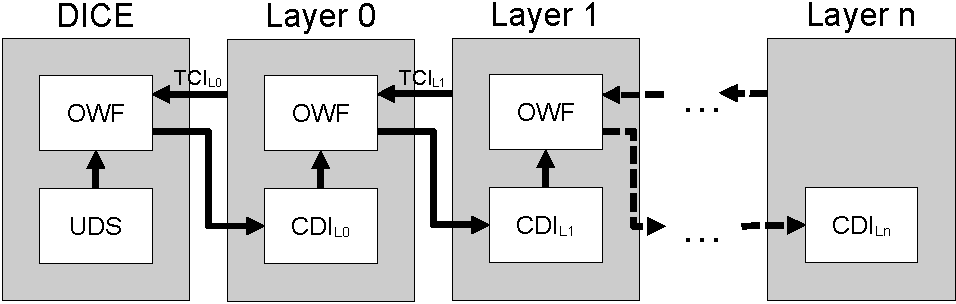
\includegraphics[width=1\linewidth]{figures/dice-layers.pdf}
  \caption{The generation of the CDIs and the certificates for each layer in a DICE architecture. Note that the diagram could be continued for an arbitrary number of layers.} \label{fig:dice-layers}
\end{figure}


The generation of the CDI values and certificates are shown in \autoref{fig:dice-layers}.
There, the CDIs and certificates are drawn where they are eventually used or what they represent, not where they are created.
E.g., CDI\textsubscript{\(n\)} and Alias Cert\textsubscript{\(n\)} are both created by layer~\(n-1\).

% Security statement

To the best of our knowledge, \ac{DICE} is so far considered a secure concept apart from physical attacks, only implementation problems can bear security problems~\cite{Jaeger2020, Hristozov2022}.

% How attestation works